%!TEX root = ../proceedings.tex
% \subsection{Vulnerable workers, and how to protect them}
\textit{Many workers in the gig economy are vulnerable to exploitation;
careless or malicious systems can endanger workers.}

At organization E, workers expressed concern when we discussed the ability to show a profile picture to customers in advance of their arrival.
These concerns stemmed from fears of their privacy being violated,
and discrimination over their race, age, gender, and other characteristics.
In particular, workers at organization E were afraid that customers would reject them for being too old.

organization E addressed this issue by emphasizing the qualifications of workers,
abstracting their names and details for first-time jobs.
Workers fundamentally have final say over whether to be matched to a customer,
based on general data about the location,
an indication of whether they've worked together before, and a rough estimate of the amount of work solicited
(In most cases, a precise estimate of how long a job will take is difficult to make without someone familiar with the work on-site to make an informed estimate).

If a customer has hired through organization E before and wants to hire a previously hired worker,
a rudimentary system allows volunteer dispatch staff to identify those workers for matching.
This allows workers to gradually develop a body of clients over time;
eventually, they no longer rely on organization E to refer customers to them at all.
Organization A utilized a similar approach, allowing customers to request a worker they've worked with in the past,
but otherwise not revealing information about workers to customers.

Many of the existing marketplaces for gig work don't expose such affordances to request a previously hired worker.
% making it difficult or impossible to grow a regular client base without leaving the system entirely.
This may be deliberate, as it effectively prevents workers from fostering a community of clients.
By preventing workers and customers from becoming familiar,
workers become dependent on the market created by the platform to provide leads on customers.
Whether a system promotes such dependence or not is up to the system's designers,
but we articulate a possible approach which makes repeat work possible.

As we illustrate in Figure ~\ref{fig:previousHire},
a simple interface exposing basic information about a previously hired worker can remind a customer whom they want to select.
Further, a technological solution such as this can ease the negotiation of scheduling;
in our case, we suggest prompting the worker for their availability.
Once several times are suggested, the customer can select and confirm a time.


\begin{figure}[t]
\centering
  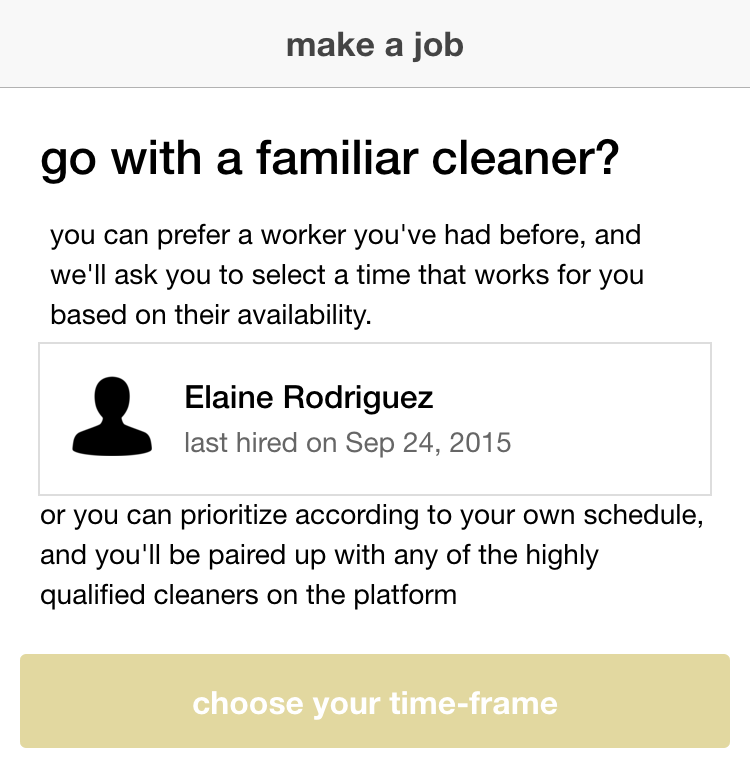
\includegraphics[width=1\columnwidth]{figures/recurrent}
    \caption{By exposing some information about previously matched workers,
    a system can facilitate workers developing a reliable customer base.}~\label{fig:previousHire}
\end{figure}

Working with organization B, nurses we spoke to expressed concern over disrespectful or uncooperative patients.
Nurses described various safety concerns including
violent neighborhoods, dangerous pets such as dogs, and patients in declining mental health.
Nurses told us that these were inherent risks associated with in-home care.
Some of the nurses that we spoke to clarified that, in cases where they felt a particular danger,
they may decline to meet a patient and communicate that concern later.

\begin{figure}[t]
\centering
  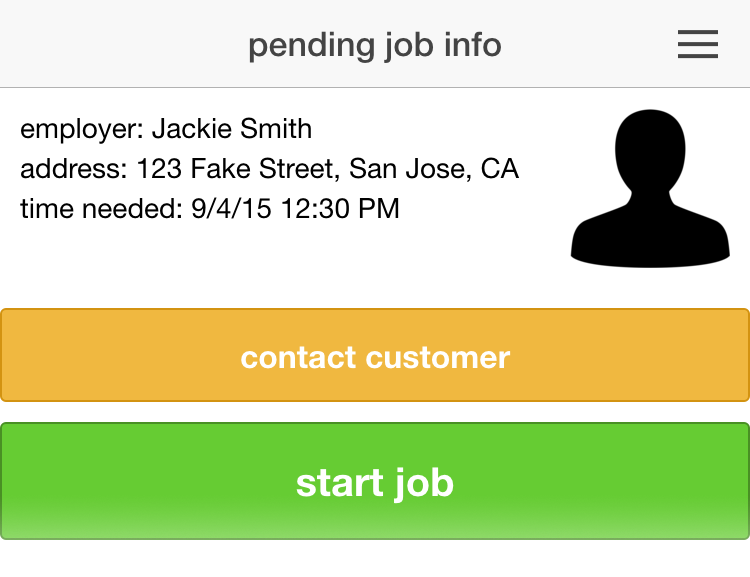
\includegraphics[width=1\columnwidth]{figures/startwork}
    \caption{A simple interface for workers,
    allowing them to contact customers,
    facilitates the resolution of potential issues before work begins,
    such as difficulty finding a location, ambiguity in instructions, etc\dots}~\label{fig:startwork}
\end{figure}

Technological systems can assist workers in cases like these;
by exposing customer contact information to workers (and potentially vice versa),
workers can contact customers before they begin work to clarify or resolve any issues.
